\documentclass{report}

\usepackage[T2A]{fontenc}
\usepackage[utf8]{luainputenc}
\usepackage[english, russian]{babel}
\usepackage[pdftex]{hyperref}
\usepackage[14pt]{extsizes}
\usepackage{listings}
\usepackage{color}
\usepackage{geometry}
\usepackage{enumitem}
\usepackage{multirow}
\usepackage{graphicx}
\usepackage{indentfirst}
\usepackage{amsmath}

\geometry{a4paper,top=2cm,bottom=3cm,left=2cm,right=1.5cm}
\setlength{\parskip}{0.5cm}
\setlist{nolistsep, itemsep=0.3cm,parsep=0pt}

\lstset{language=C++,
		basicstyle=\footnotesize,
		keywordstyle=\color{blue}\ttfamily,
		stringstyle=\color{red}\ttfamily,
		commentstyle=\color{green}\ttfamily,
		morecomment=[l][\color{magenta}]{\#}, 
		tabsize=4,
		breaklines=true,
  		breakatwhitespace=true,
  		title=\lstname,       
}

\makeatletter
\renewcommand\@biblabel[1]{#1.\hfil}
\makeatother

\begin{document}

\begin{titlepage}

\begin{center}
Министерство науки и высшего образования Российской Федерации
\end{center}

\begin{center}
Федеральное государственное автономное образовательное учреждение высшего образования \\
Национальный исследовательский Нижегородский государственный университет им. Н.И. Лобачевского
\end{center}

\begin{center}
Институт информационных технологий, математики и механики
\end{center}

\vspace{4em}

\begin{center}
\textbf{\LargeОтчет по лабораторной работе} \\
\end{center}
\begin{center}
\textbf{\Large«Поразрядная сортировка для вещественных чисел 
(тип double) с простым слиянием.»} \\
\end{center}

\vspace{4em}

\newbox{\lbox}
\savebox{\lbox}{\hbox{text}}
\newlength{\maxl}
\setlength{\maxl}{\wd\lbox}
\hfill\parbox{7cm}{
\hspace*{5cm}\hspace*{-5cm}\textbf{Выполнил:} \\ студент группы 381806-4 \\ Григорян Г.А.\\
\\
\hspace*{5cm}\hspace*{-5cm}\textbf{Проверил:}\\ доцент кафедры МОСТ, \\ кандидат технических наук \\ Сысоев А. В. \\
}
\vspace{\fill}

\begin{center} Нижний Новгород \\ 2020 \end{center}

\end{titlepage}

\setcounter{page}{2}

% Содержание
\tableofcontents
\newpage

% Постановка задачи
\section*{Постановка задачи}
\addcontentsline{toc}{section}{Постановка задачи}
Требуется реализовать линейную и параллельную поразрядную сортировку вещественных чисел (типа double) с простым слиянием при помощи языка C++, а также сравнить время выполнения на разном количестве запускаемых процессов.
\newpage

% Метод решения
\section*{Метод решения}
\addcontentsline{toc}{section}{Метод решения}
Поразрядная сортировка имеет две модификации: Most Significant Digit (MSD) и Least Significant Digit (LSD). В данной работе будет рассмотрен алгоритм LSD, так как данный алгоритм является наиболее эффективным. Идея поразрядной восходящей сортировки (Least Significant Digit (LSD) Radix Sort) заключается в том, что выполняется последовательная сортировка чисел по разрядам (от младшего разряда к старшему). 

Рассмотрим алгоритм работы сортировки на примере массива десятичных чисел из 9 элементов:

\begin{figure}[htp]
    \centering
    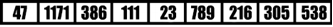
\includegraphics[width=14cm]{images/image1.png}
    \label{fig:galaxy}
\end{figure}

На первой итерации сортировки выполняется размещение элементов в отсортированном порядке по младшему разряду чисел:

\begin{figure}[htp]
    \centering
    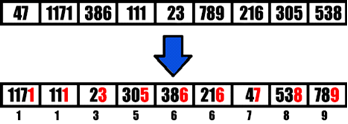
\includegraphics[width=14cm]{images/image2.png}
    \label{fig:galaxy}
\end{figure}

Примечание: в последующих иллюстрациях красным цветом будут выделены разряды чисел, по которым происходит сортировка.


На следующей итерации происходит сортировка элементов по второму разряду:

\begin{figure}[htp]
    \centering
    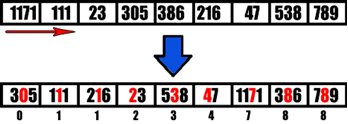
\includegraphics[width=10cm]{images/image3.png}
    \label{fig:galaxy}
\end{figure}
\newpage
Примечание: красная стрелка указывает направление алгоритма (т.е мы движемся от левого края к правому краю массива).

Далее выполняется упорядочивание элементов по третьему разряду:

\begin{figure}[htp]
    \centering
    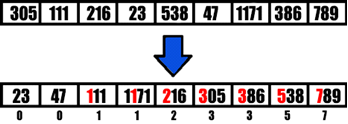
\includegraphics[width=14cm]{images/image4.png}
    \label{fig:galaxy}
\end{figure}

На последнем шаге выполняется сортировка по старшему разряду:

\begin{figure}[htp]
    \centering
    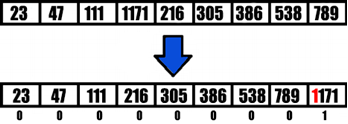
\includegraphics[width=14cm]{images/image5.png}
    \label{fig:galaxy}
\end{figure}

Поразрядная сортировка массива будет работать только в том случае, если
сортировка, выполняющаяся по разряду, является устойчивой (элементы равных разрядов не будут менять взаимного расположения при сортировке по очередному размеру): 


\begin{figure}[htp]
    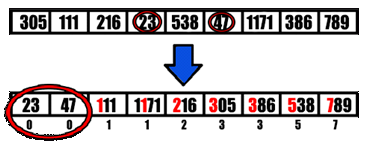
\includegraphics[width=9cm]{images/image6.png}
    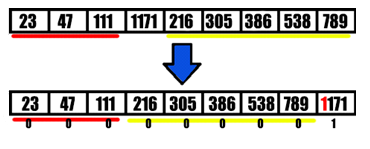
\includegraphics[width=9cm]{images/image7.png}
    \label{fig:galaxy}
\end{figure}
Примечание: приведены два примера устойчивого расположение чисел при поразрядной сортировке.

\newpage

Современные процессоры предназначены для обработки данных, которые
представлены в битах и байтах, поэтому выполнять сортировку по десятичным
разрядам чисел не эффективно. Рассмотрим побайтовую реализацию
поразрядной сортировки, т.е. будем рассматривать число как набор 256-
значных цифр. В таком случае для сортировки разряда будет удобно
использовать сортировку подсчетом (с модификацией, которая не будет
менять взаимного расположения элементов равных разрядов).
Сортировка подсчетом по i-му байту будет проходить в два прохода по
исходному массиву:

1.	При первом проходе по исходному массиву выполняется подсчет
i-ых байт в массиве mas, результат будет сохранен в массив подсчетов
counter из 256 элементов;

2.	В массив counters на основании посчитанных данных выполняется
подсчет смещений, по которым будут сохраняться элементы:
counters [0] =0 для всех j от 1 до 255 counters [j]= counters [pmem[8 * i + offset]]++;]

3.	При втором проходе по исходному массиву mas выполняется
копирование элемента во вспомогательный массив по соответствующему индексу в массиве смещений counters и выполняется
инкремент смещения.

Вещественный тип представляется в памяти так (рассмотрим 8-байтовый тип double), что число кодируется следующим образом: 

\begin{figure}[htp]
    \centering
    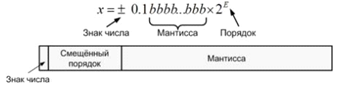
\includegraphics[width=14cm]{images/image8.png}
    \label{fig:galaxy}
\end{figure}
Поразрядная сортировка таких чисел будет выполняться в 8 проходов, начинаяот младшего байта до старшего.


\newpage

% Описание схемы распараллеливания
\section*{Описание схемы распараллеливания}
\addcontentsline{toc}{section}{Описание схемы распараллеливания}

\par Можно выделить два подхода к реализации параллельного алгоритма сортировки: внутренняя реализация параллельного алгоритма или внешнее распараллеливание за счет слияния отсортированных частей.
\parАлгоритм побайтовой восходящей сортировки заключается в последовательном применении сортировки подсчетом к каждому байту чисел, поэтому параллельно может выполняться только сортировка подсчетом для каждого байта. При этом параллельная версия сортировки подсчетом должна сохраняться свойство устойчивости сортировки (а это тяжелая задача).
\par Идея параллельной реализации с использованием слияния заключается в выполнении следующих шагов:

1. Сортировка частей массива.
\par2. Слияние отсортированных частей массива.

\par Сортировка частей массива может выполняться без каких-либо синхронизаций, поэтому теоретическое ускорение этого этапа является линейным. Этап слияние в зависимости от алгоритма может иметь различную эффективность.

\par Идея простого слияния заключается в том, что один поток может выполнять слияние двух отсортированных массивов по классическому алгоритму. В этом случае слияние n массивов могут выполнять n/2 параллельных потоков. На следующем шаге слияние n/2 полученных массивов будут выполнять n/4 потоков и т.д. Таким образом, последнее слияние будет выполнять один поток, а учитывая, что сортировка частей массива имеет линейную трудоемкость, то слияние вносит существенный вклад во время работы алгоритма.

\begin{figure}[htp]
    \centering
    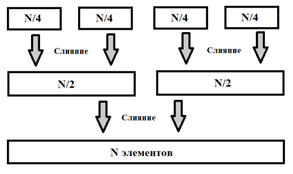
\includegraphics[width=10cm]{images/image9.png}
    \label{fig:galaxy}
\end{figure}

\newpage

% Подтверждение корректности
\section*{Подтверждение корректности}
\addcontentsline{toc}{section}{Подтверждение корректности}

\par Для подтверждения корректности в программе реализована функция автоматической проверки isSorted(), которая принимает на вход результат работы двух алгоритмов: последовательного и параллельного. Функция возвращает true, если оба алгоритма прошли проверку. Функция возвращает false в случае, если какой-либо из алгоритмов был некоректен. Если подтверждается корректность программы, то все google test проходят должным образом.

\newpage
% Описание программной реализации
\section*{Описание программной реализации}
\addcontentsline{toc}{section}{Описание программной реализации}

\par Для запуска используется обычный способ, характерный для всех программ, написанных с использованием технологии MPI. Соответственно команда для запуска через командную строку имеет следующий вид:

\begin{figure}[htp]
    \centering
    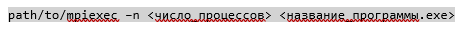
\includegraphics[width=15cm]{images/put.png}
    \label{fig:galaxy}
\end{figure}

\par Программа выводит время google test и соответствующее время последовательного и параллельного алгоритма.

\begin{figure}[htp]
    \centering
    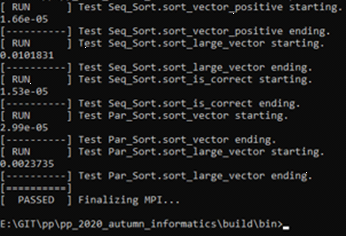
\includegraphics[width=10cm]{images/image10.png}
    \label{fig:galaxy}
\end{figure}

\begin{itemize}

\item getRandomVector – функция для заполнения массива случайными значениями. 
\item isSorted – функция, проверяющая отсортированность массива.
\item passing – функция побайтовой сортировки.
\item lastPassing – функция проверки побайтовой сортировки в последней итерации.
\item orderedmerge – функция слияния 2-х массивов.
\item seqSorting – функция последовательного алгоритма.
\item parSorting – функция параллельного алгоритма.

\end{itemize}
\newpage

% Результаты экспериментов
\section*{Результаты экспериментов}
\addcontentsline{toc}{section}{Результаты экспериментов}
Эксперименты проводились на ПК со следующими характеристиками:

\begin{itemize}
\item Процессор AMD Ryzen 3 2200g with Radeon Vega Graphics 3.85 Ghz
\item Оперативная память: 8,00ГБ DDR4
\item ОС: Microsoft Windows 10 Home
\end{itemize}

\par Рассмотрим приведённую ниже таблицу для оценки результатов:
\\


\begin{figure}[htp]
    \centering
    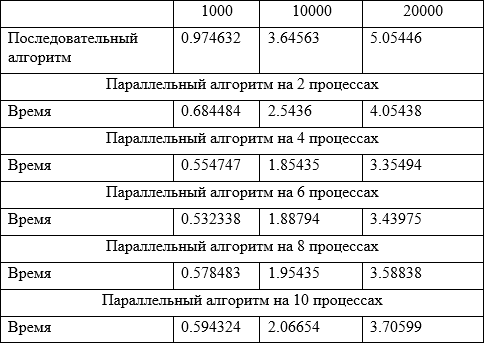
\includegraphics[width=10cm]{images/tt.png}
    \label{fig:galaxy}
\end{figure}


\par Результаты вычислительных экспериментов приведены ниже:

\begin{figure}[htp]
    \centering
    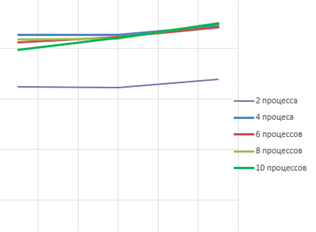
\includegraphics[width=10cm]{images/image11.png}
    \label{fig:galaxy}
\end{figure}

\newpage

% Заключение
\section*{Заключение}
\addcontentsline{toc}{section}{Заключение}
\par Была реализована последовательная и параллельная реализация поразрядной сортировки вещественных чисел с простым слиянием. Было замерено время работы этих сортировок, эффективность и протестирована их корректность. В результате было выяснено, что последовательная версия от параллельной по времени почти не различается (каких-либо серьезных различий не было выявлено). Это говорит нам о том, что параллельная реализация является неэффективна по сравнению с последовательной.

\newpage

% Литература
\begin{thebibliography}{1}
\addcontentsline{toc}{section}{Литература}

\bibitem{Sidnev}Сиднев А.А., Сысоев А.В., Мееров И.Б. Учебный курс «Технологии параллельного программирования»

\bibitem{Sidnev1}Сиднев А.А., Сысоев А.В., Мееров И.Б. Параллельные численные методы: «Лабораторная работа: Сортировки».

\end{thebibliography}
\newpage

% Приложение
\section*{Приложение}
\addcontentsline{toc}{section}{Приложение}
В данном разделе находится листинг всего кода, написанного в рамках лабораторной работы.
\begin{lstlisting}
// Copyright 2020 Grigoryan Garry
#ifndef MODULES_TASK_3_GRIGORYAN_G_DOUBLE_SORTING_SORT_H_
#define MODULES_TASK_3_GRIGORYAN_G_DOUBLE_SORTING_SORT_H_

std::vector<double> getRandomVector(double sz);
bool is_sorted(double* source, int size);
void passing(double* source, double* dest, int size, int offset);
void last_passing(double* source, double* dest, int size, int offset);
void ordered_merge(double* source1, int size1, double* source2, int size2, double* dest);
void seq_sorting(double* source, int size);
void par_sorting(double** source, int size);

#endif  // MODULES_TASK_3_GRIGORYAN_G_DOUBLE_SORTING_SORT_H_

\end{lstlisting}
\newpage
\begin{lstlisting}
// Copyright 2020 Grigoryan Garry
#include <mpi.h>
#include <vector>
#include <string>
#include <random>
#include <ctime>
#include <algorithm>
#include <vector>
#include "../../../modules/task_3/grigoryan_g_double_sorting/sort.h"

std::vector<double> getRandomVector(double sz) {
	std::mt19937 gen;
	gen.seed(static_cast<unsigned int>(time(0)));
	std::vector<double> vec(sz);
	for (int i = 0; i < sz; i++) { vec[i] = gen() % 100; }
	return vec;
}


bool is_sorted(double* source, int size) {
  for (int i = 0; i < size - 1; i++) {
    if (source[i + 1] < source[i]) {
      return false;
    }
  }
  return true;
}

void passing(double* source, double* dest, int size, int offset) {
  unsigned char* pmem = (unsigned char*)source;
  int counters[256];
  int sum = 0;

  for (int i = 0; i < 256; i++) counters[i] = 0;

  for (int i = 0; i < size; i++) counters[pmem[8 * i + offset]]++;

  for (int i = 0; i < 256; i++) {
    int tmp = counters[i];
    counters[i] = sum;
    sum += tmp;
  }

  for (int i = 0; i < size; i++) {
    int index = 8 * i + offset;
    dest[counters[pmem[index]]] = source[i];
    counters[pmem[index]]++;
  }
}

void last_passing(double* source, double* dest, int size, int offset) {
  unsigned char* pmem = (unsigned char*)source;
  int counters[256];
  int sum = 0;

  for (int i = 0; i < 256; i++) counters[i] = 0;

  for (int i = 255; i > 127; i--) {
    counters[i] += sum;
    sum = counters[i];
  }

  for (int i = 0; i < 128; i++) {
    int tmp = counters[i];
    counters[i] = sum;
    sum += tmp;
  }

  for (int i = 0; i < size; i++) {
    int index = 8 * i + offset;
    if (pmem[index] < 128) {
      dest[counters[pmem[index]]] = source[i];
      counters[pmem[index]]++;
    } else {
      counters[pmem[index]]--;
      dest[counters[pmem[index]]] = source[i];
    }
  }
}

void ordered_merge(double* source1, int size1, double* source2, int size2, double* dest) {
  int i = 0, j = 0, k = 0;

  while ((i < size1) && (j < size2)) {
    if (source1[i] < source2[j]) {
      dest[k] = source1[i];
      i++;
    } else {
      dest[k] = source2[j];
      j++;
    }
    k++;
  }
  while (i < size1) {
    dest[k] = source1[i];
    i++;
    k++;
  }
  while (j < size2) {
    dest[k] = source2[j];
    j++;
    k++;
  }
}

void seq_sorting(double* source, int size) {
  double* temp = NULL;
  double* dest = new double[size];
  for (int i = 0; i < 8; i++) {
    passing(source, dest, size, i);
    temp = source;
    source = dest;
    dest = temp;
  }
  last_passing(source, dest, size, 7);
  delete[] dest;
}

void par_sorting(double** source, int size) {
  int proc_rank = 0, proc_size = 0;
  MPI_Comm_size(MPI_COMM_WORLD, &proc_size);
  MPI_Comm_rank(MPI_COMM_WORLD, &proc_rank);

  int lenght = size / proc_size, addition = size % proc_size;

  double* dest = NULL;
  double* temp = NULL;
  if (0 == proc_rank) {
    dest = new double[lenght + addition];
    temp = new double[size];
  } else {
    dest = new double[lenght];
  }
  int* displs = new int[proc_size];
  int* scounts = new int[proc_size];

  displs[0] = 0;
  scounts[0] = lenght + addition;
  for (int i = 1; i < proc_size; i++) {
    displs[i] = addition + lenght * i;
    scounts[i] = lenght;
  }

  MPI_Scatterv(*source, scounts, displs, MPI_DOUBLE, dest, scounts[proc_rank], MPI_DOUBLE, 0, MPI_COMM_WORLD);
  seq_sorting(dest, scounts[proc_rank]);
  MPI_Gatherv(dest, scounts[proc_rank], MPI_DOUBLE, temp, scounts, displs, MPI_DOUBLE, 0, MPI_COMM_WORLD);

  if (0 == proc_rank) {
    double* tmp = NULL;

    for (int i = 0; i < proc_size - 1; i++) {
      ordered_merge(temp, displs[i + 1], &temp[displs[i + 1]], scounts[i + 1], *source);
      tmp = *source;
      *source = temp;
      temp = tmp;
    }
    tmp = *source;
    *source = temp;
    temp = tmp;
  }
  delete[] dest;
  delete[] temp;
  delete[] displs;
  delete[] scounts;
}


\end{lstlisting}
\newpage
\begin{lstlisting}
// Copyright 2020 Grigoryan Garry
#include <gtest-mpi-listener.hpp>
#include <gtest/gtest.h>

#include "./sort.h"

TEST(Seq_Sort, sort_vector_positive) {
  int rank = 0;
  MPI_Comm_rank(MPI_COMM_WORLD, &rank);

  if (0 == rank) {
    int size = 9;
    double *vector = new double[size] { 4.0, 9.66057, 1.69, 99.147, 57.3579, 34.23, 44.43, 432.5435, 9.6 };
    bool result = false;
    double start = MPI_Wtime();
    seq_sorting(vector, size);
    double finish = MPI_Wtime();
    result = is_sorted(vector, size);
    ASSERT_EQ(true, result);
    std::cout << finish - start << std::endl;
  }
}

TEST(Seq_Sort, sort_large_vector) {
  int rank = 0;
  MPI_Comm_rank(MPI_COMM_WORLD, &rank);

  if (0 == rank) {
     int size = 10000;
     double *vector = new double[size];
     for (int i = 0; i < size; i++) vector[i] = (size - i) * 0.001 + (i + size / 2);
    bool result = false;
     double start = MPI_Wtime();
    seq_sorting(vector, size);
    result = is_sorted(vector, size);
    double finish = MPI_Wtime();
    ASSERT_EQ(true, result);
    std::cout << finish - start << std::endl;
  }
}

TEST(Seq_Sort, sort_is_correct) {
  int rank = 0;
  MPI_Comm_rank(MPI_COMM_WORLD, &rank);

  if (0 == rank) {
    int size = 5;
    double *result = new double[size] { 1.69, 2.0, 8.66667, 57.3579, 99.147};
    double *vector = new double[size] { 2.0, 8.66667, 1.69, 99.147, 57.3579 };
    double start = MPI_Wtime();
    seq_sorting(vector, size);
    double finish = MPI_Wtime();
    for (int i = 0; i < size; i++) {
      ASSERT_NEAR(result[i], vector[i], 0.01);
    }
    std::cout << finish - start << std::endl;
  }
}

TEST(Par_Sort, sort_vector) {
  int rank = 0;
  MPI_Comm_rank(MPI_COMM_WORLD, &rank);
  int size = 9;
  double *vector = new double[size] { 99.147, 9.66057, 1.69, 4.0, 57.3579, 34.23, 44.43, 432.5435, 96.005 };
  double start = MPI_Wtime();
  par_sorting(&vector, size);
  double finish = MPI_Wtime();
  if (0 == rank) {
    bool result = false;
    result = is_sorted(vector, size);
    ASSERT_EQ(true, result);
    std::cout << finish - start << std::endl;
  }
  delete[] vector;
}

TEST(Par_Sort, sort_large_vector) {
  int rank = 0;
  MPI_Comm_rank(MPI_COMM_WORLD, &rank);
  int size = 10000;
  double *vector = new double[size];
  for (int i = 0; i < size; i++) vector[i] = (size - i) * 0.001 + (i + size / 2);
  double start = MPI_Wtime();
  par_sorting(&vector, size);
  double finish = MPI_Wtime();
  if (0 == rank) {
    bool result = false;
    result = is_sorted(vector, size);
    ASSERT_EQ(true, result);
    std::cout << finish - start << std::endl;
  }
  delete[] vector;
}


int main(int argc, char** argv) {
  ::testing::InitGoogleTest(&argc, argv);
  MPI_Init(&argc, &argv);

  ::testing::AddGlobalTestEnvironment(new GTestMPIListener::MPIEnvironment);
  ::testing::TestEventListeners& listeners =
    ::testing::UnitTest::GetInstance()->listeners();

  listeners.Release(listeners.default_result_printer());
  listeners.Release(listeners.default_xml_generator());

  listeners.Append(new GTestMPIListener::MPIMinimalistPrinter);
  return RUN_ALL_TESTS();
}


\end{lstlisting}
\end{document}